
\documentclass{beamer}

\usepackage{algpseudocode, color, colortbl, listings, MnSymbol}

\usepackage{hyperref}
\hypersetup{
    colorlinks=true,
    urlcolor=blue,
}

\usetheme{Montpellier}
\usecolortheme{rose}

% page numbers, from
% https://tex.stackexchange.com/questions/137022/how-to-insert-page-number-in-beamer-navigation-symbols
\expandafter\def\expandafter\insertshorttitle\expandafter{%
  \insertshorttitle\hfill%
  \insertframenumber\,/\,\inserttotalframenumber}

\definecolor{Gray}{gray}{0.8}
\newcolumntype{g}{>{\columncolor{Gray}}c}

\newcommand{\stanza}{ \\~\ }

\title{13. Dynamic Programming for Longest Common Subsequence}
\subtitle{CPSC 535}
\author{Kevin A. Wortman}
\institute{ 
\includegraphics[height=2cm]{csuf-logo-cmyk} }
\date{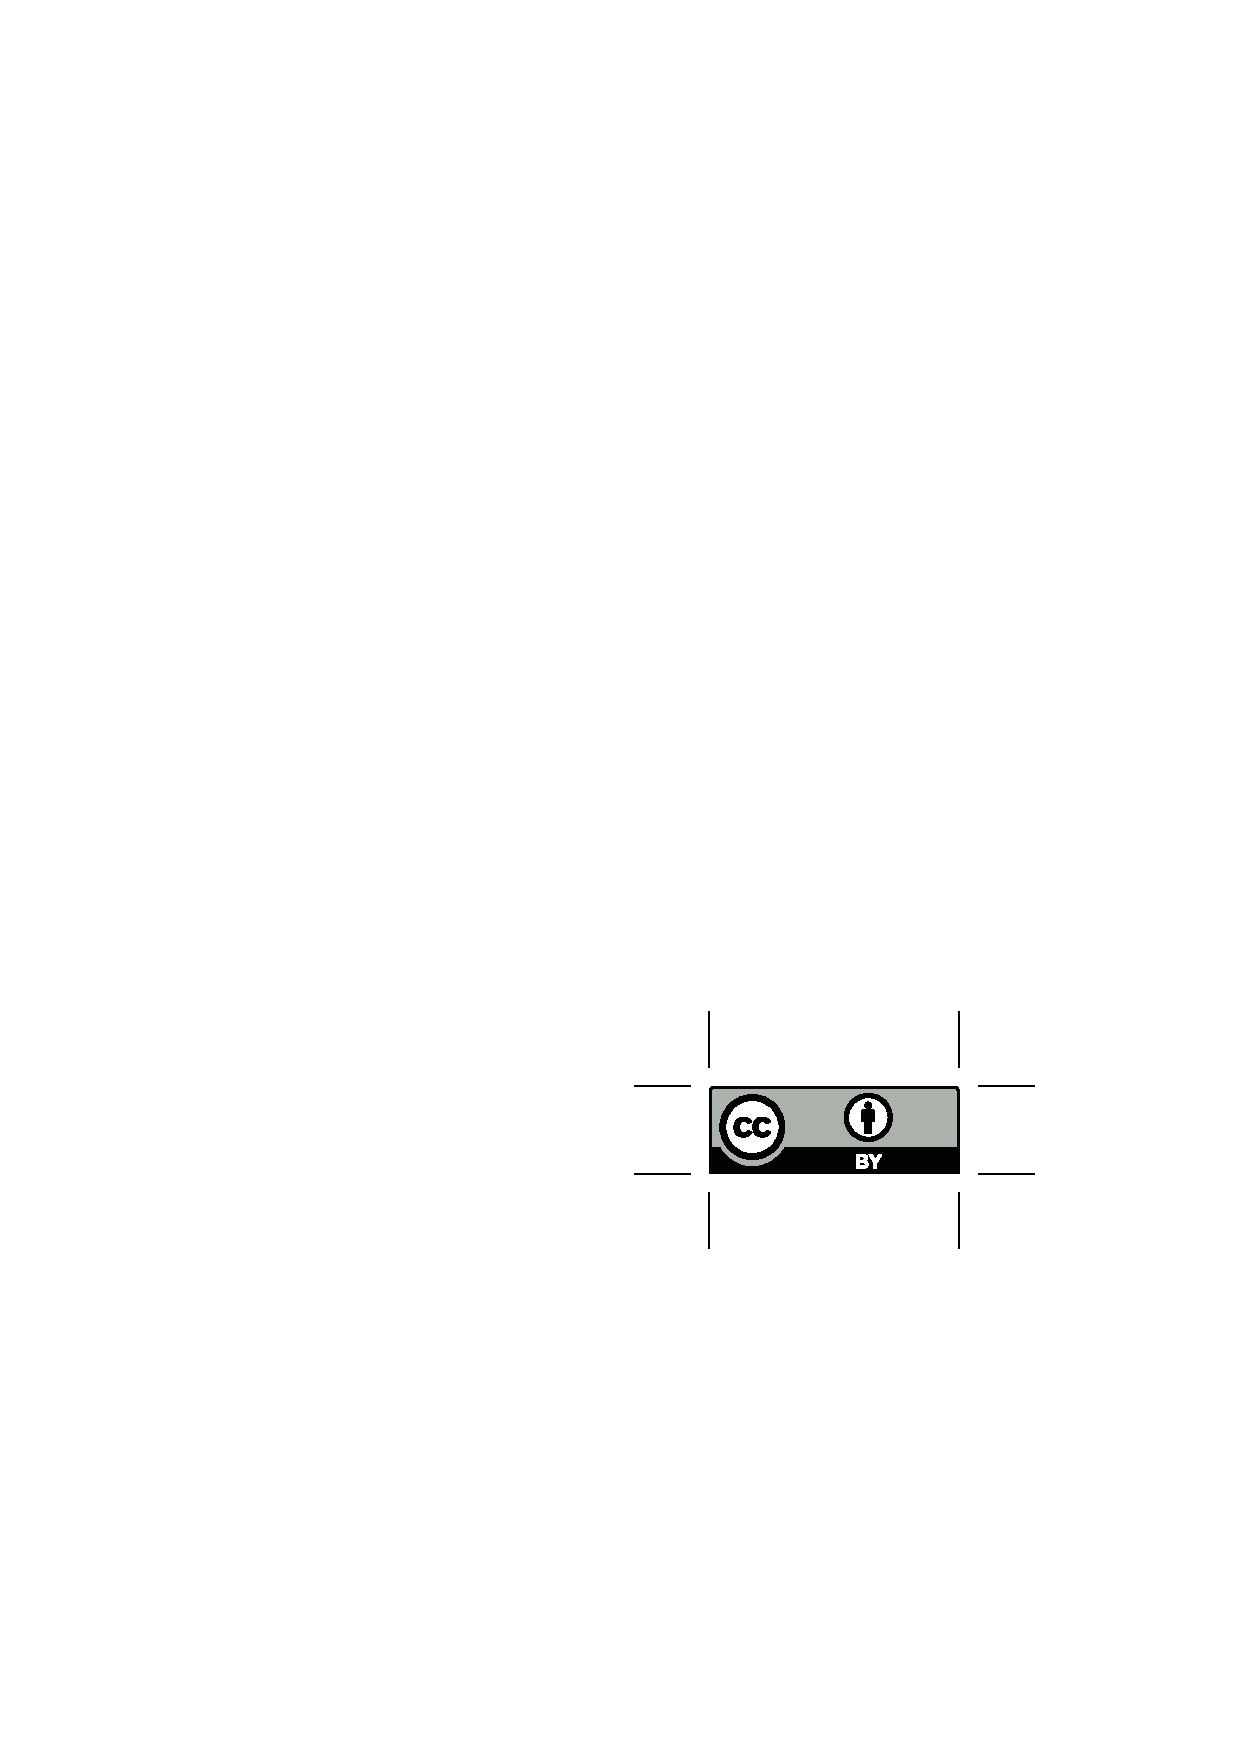
\includegraphics[height=14pt]{by} \\

{\tiny
This work is licensed under a
\href{http://creativecommons.org/licenses/by/4.0/}{Creative Commons Attribution 4.0 International License}.
}}

\begin{document}

\begin{frame}
  \titlepage
\end{frame}

\begin{frame} \frametitle{Big Idea: Alternative Kinds of Solutions}
  \begin{itemize}
  \item So far
    \begin{itemize}
      \item Step 2. Derive a \textbf{recurrence} for an optimal value.
      \item Recall rod cutting:
        \[ r_i = \max_{1 \leq i \leq n} (p_i + r_{n-i}) \]
      \item Recall matrix chain multiplication:
        \[ r_{i, j} = \min_{i \leq k \leq \, j} r_{i, k} + r_{k+1, \, j} + p_{i-1} p_k p_j \]
    \end{itemize}
  \item Now: longest common subsequence (LCS)
    \begin{itemize}
      \item not simply minimizing/maximizing one expression
      \item instead, choose between \textbf{three alternatives}
      \item \textbf{2D table}, like matrix chain
    \end{itemize}
  \end{itemize}
\end{frame}

\begin{frame} \frametitle{Subsequences}
  \begin{itemize}
  \item Let $X=\langle x_1, x_2, \ldots, x_m \rangle$ and $Y=\langle y_1, y_2, \ldots, y_n \rangle$ be two sequences
  \item Define \textbf{prefix} notation: $X_k = \langle x_1, \ldots, x_k \rangle; X_0 = \langle \rangle$
  \begin{itemize}
    \item if $X=\langle 2, 7, 8, 1, 7, 1, 2 \rangle$ then $X_3 = \langle 2, 7, 8 \rangle $
  \end{itemize}
  \item Informally: a \textbf{subsequence} of $Y$ is a copy of $Y$ with some elements removed
  \item Formally: $X$ is a \textbf{subsequence} of $Y$ if there exists an increasing sequence of indices $\langle i_1, i_2, \ldots, i_k \rangle$ such that, for all $j \in [1, k], x_j = y_{i_j}$
  \item Example: for $X=\langle B, C, D, B\rangle$ and $Y=\langle A, B, C, B, D, A, B \rangle,$ $X$ is a subsequence of $Y$ with index sequence $\langle 2, 3, 5, 7 \rangle$
  \end{itemize}
\end{frame}

\begin{frame} \frametitle{Common Subsequence}
  \begin{itemize}
  \item $Z$ is a \textbf{common subsequence} of $X$ and $Y,$ if $Z$ is a subsequence $X$ and $Z$ is a subsequence of $Y$
  \item a \textbf{longest common subsequence} is a common subsequence of maximum length
  \item Example: let $X=\langle A, B, C, B, D, A, B \rangle $  and $Y=\langle B, D, C, A, B, A \rangle$ 
  \item $Z=\langle B, C, A \rangle$ is a common subsequence
  \item $Z=\langle B, C, B, A \rangle$ is a longest common subsequence
  \end{itemize}
\end{frame}

\begin{frame} \frametitle{Longest Common Subsequence}

  \emph{Longest Common Subsequence (LCS) solution problem} \\
  \textbf{input:} sequences $X=\langle x_1, x_2, \ldots, x_m \rangle$ and $Y=\langle y_1, y_2, \ldots, y_n \rangle$
  \textbf{output:} a longest common subsequence of $X$ and $Y$ \stanza
  
  \emph{Longest Common Subsequence (LCS) value problem} \\
  \textbf{input:} (same) \\
  \textbf{output:} the length of a longest common subsequence of $X$ and $Y$ \stanza

\end{frame}

\begin{frame} \frametitle{Design Process}
  \begin{enumerate}
    \item Identify the problem's \textbf{solution} and \textbf{value}, and note which is our \textbf{goal}.
    \item Derive a \textbf{recurrence} for an optimal value.
    \item Design a divide-and-conquer algorithm that computes an \textbf{optimal value}.
    \item Design a dynamic programming algorithm that computes an \textbf{optimal value}.
    \begin{enumerate}
      \item \textbf{top-down} alternative: add table base case (\textbf{memoization})
      \item \textbf{bottom-up} alternative: rewrite to use bottom-up loops instead of recursion
    \end{enumerate}
    \item (if goal is a solution algo.) Design a dynamic programming algorithm that computes an \textbf{optimal solution}.
  \end{enumerate}
  \end{frame}

  \begin{frame} \frametitle{Longest Common Subsequence Step 1}
    \begin{enumerate}
      \item Identify the problem's \textbf{solution} and \textbf{value}, and note which is our \textbf{goal}.
      \stanza
    \end{enumerate}

    \begin{itemize}
      \item \textbf{solution:} a sequence e.g. $\langle B, C, B, A \rangle$
      \item \textbf{value:} integer length of a sequence e.g. 4
      \item eventual goal is solution
      \item start with value
    \end{itemize}
  \end{frame}
  
  \begin{frame} \frametitle{Longest Common Subsequence Step 2}
    \begin{enumerate}
      \setcounter{enumi}{1}
      \item Derive a \textbf{recurrence} for an optimal value.
      \stanza
    \end{enumerate}
    \begin{itemize}
      \item Recall input: $X=\langle x_1, x_2, \ldots, x_m \rangle$ and $Y=\langle y_1, y_2, \ldots, y_n \rangle$
      \item Recall \emph{prefix:} $X_i$ is first $i$ elements of $X$
      \item Define $LCS(X, Y) \equiv$ length of longest common subsequence of $X$ and $Y$
      \item We need to define $LCS$ recursively
      \end{itemize}

      \end{frame}
      \begin{frame} \frametitle{Longest Common Subsequence Step 2}
        \begin{enumerate}
          \setcounter{enumi}{1}
          \item Derive a \textbf{recurrence} for an optimal value.
          \stanza
        \end{enumerate}
        \begin{itemize}
          \item \textbf{Idea:} If last symbols $x_m=y_n$ match, then extend a shorter common subsequence:
            $LCS(X, Y) = LCS(X_{m-1}, Y_{n-1}) + 1$
          \item Else ($x_m \ne y_n$), have to omit $x_m$ or $y_n$
            \begin{itemize}
            \item Omit $x_m$: $LCS(X, Y) = LCS(X_{m-1}, Y)$
            \item Omit $y_n$: $LCS(X, Y) = LCS(X, Y_{n-1})$
            \item Want \textbf{longest} so 
            \[ LCS(X, Y) = \max(LCS(X_{m-1}, Y), LCS(X, Y_{n-1})) \]
              \end{itemize}
          \end{itemize}
    \end{frame}

    \begin{frame} \frametitle{Example}
      \begin{itemize}
        \item Suppose $X=\langle A, B, A, D \rangle$ and $Y = \langle B, B, A, C, D \rangle$
        \item Last symbols match,  $x_4=y_5=D,$ so
          \begin{align*}
            LCS(X,Y) &= LCS(X_{m-1}, Y_{n-1}) + 1 \\
            &= LCS(\langle A, B, A \rangle, \langle B, B, A, C \rangle) + 1
          \end{align*}
        \item Now suppose $X=\langle A, B, A, D \rangle$ and $Y = \langle B, B, A, C, C \rangle$
        \item Last symbols differ ($x_4=D$ but $y_5=C$), so
          {\footnotesize
          \begin{align*}
            LCS(X,Y)
            &= \max(LCS(X_{m-1}, Y_n), LCS(X_m, Y_{n-1})) \\
            &= \max(\langle A, B, A \rangle, \langle B, B, A, C, C \rangle), LCS(\langle A, B, A, D \rangle, \langle B, B, A, C \rangle)) 
          \end{align*}
          }
        \end{itemize}
        
    \end{frame}
    
  \begin{frame} \frametitle{Longest Common Subsequence Step 2}
    \begin{enumerate}
      \setcounter{enumi}{1}
      \item Derive a \textbf{recurrence} for an optimal value.
      \stanza
    \end{enumerate}

\[ LCS(X_m, Y_n) =
    \begin{cases}
      0 & m=0 \\
      0 & n=0 \\
      LCS(X_{m-1}, Y_{n-1}) + 1 & x_m=x_n \\
      \max(LCS(X_{m-1}, Y_n), LCS(X_m, Y_{n-1})) & \text{otherwise}
    \end{cases}
  \]
  \end{frame}

  \begin{frame} \frametitle{Longest Common Subsequence Step 3}
    \begin{enumerate}
      \setcounter{enumi}{2}
      \item Design a divide-and-conquer algorithm that computes an \textbf{optimal value}.
      \stanza
    \end{enumerate}
  
    {\scriptsize
    \begin{algorithmic}[1]
      \Function{LCS-DC}{$X[1..m], Y[1..n]$}
      \If{ $m==0$ or $n==0$ }
        \State \Return{ 0 }
      \ElsIf{ $X[m] == Y[n]$ }
        \State \Return{ $\text{LCS-DC}(X[1..m-1], Y[1..n-1]) + 1$ }
      \Else
        \State \Return{ $\max(\text{LCS-DC}(X[1..m-1], Y[1..n]), \text{LCS-DC}(X[1..m], Y[1..n-1])$ }
      \EndIf
      \EndFunction
    \end{algorithmic}
    }
  \end{frame}
    
  \begin{frame} \frametitle{Matrix Chain Multiplication Step 4.a}
    \begin{enumerate}
      \setcounter{enumi}{3}
      \item Design a dynamic programming algorithm that computes an \textbf{optimal value}.
      \begin{enumerate}
        \item \textbf{top-down} alternative: add table base case (\textbf{memoization})
        \stanza
      \end{enumerate}
  \end{enumerate}

  \begin{itemize}
    \item Recall \textbf{memoization:} use a hash dictionary to make a ``memo'' of pre-calculated solutions
    \item create hash table $T$
    \item use pair $(m, n)$ as key in table $T,$ storing $LCS(X_m, Y_n)$
  \end{itemize}
  
\end{frame}  

\begin{frame} \frametitle{Matrix Chain Multiplication Step 4.a}
  {\scriptsize
  \begin{algorithmic}[1]
    \Function{LCS-MEMOIZED}{$X[1..m], Y[1..n]$}
    \State HASH-TABLE-CREATE($T$)
    \State \Return{LCS-M($T, X, Y$)}
    \EndFunction
    \Function{LCS-M}{$T, X[1..m], Y[1..n]$}
    \State $q = $ HASH-TABLE-SEARCH($T, (m, n)$)
    \If{ $q \ne$ NIL }
      \State \Return{ $q$ }
    \EndIf
    \If{ $m==0$ or $n==0$ }
      \State $q=0$
    \ElsIf{ $X[m] == Y[n]$ }
      \State $q = \text{LCS-M}(T, X[1..m-1], Y[1..m-1]) + 1$
    \Else
      \State $q = \max(\text{LCS-M}(X[1..m-1], Y[1..n]), \text{LCS-M}(X[1..m], Y[1..n-1])$
    \EndIf
    \State $q.key = (m, n)$
    \State HASH-TABLE-INSERT($q$)
    \State \Return{$q$}
    \EndFunction
  \end{algorithmic}
  }
\end{frame}

\begin{frame} \frametitle{Memoized Algorithm Analysis}
  \begin{itemize}
    \item $T$ contains $\Theta(n^2)$ pairs $(m, n)$
    \item each entry is inserted exactly once
    \item in the general case, LCS-M takes $\Theta(1)$ expected time
    \item $\Rightarrow$ LCS-MEMOIZED takes $\Theta(n^2)$ expected time
  \end{itemize}
\end{frame}

\begin{frame} \frametitle{Longest Common Subsequence Step 4.b}
  \begin{enumerate}
    \setcounter{enumi}{3}
    \item Design a dynamic programming algorithm that computes an \textbf{optimal value}.
    \begin{enumerate}
      \item \textbf{top-down} alternative: add table base case (\textbf{memoization})
      \item \textbf{bottom-up} alternative: rewrite to use bottom-up loops instead of recursion
      \stanza
    \end{enumerate}
\end{enumerate}

\begin{itemize}
  \item create 2D array $c$ where $c[i][\, j] = LCS(X_i, Y_j)$
  \item \textbf{bottom-up:} write an explicit \textbf{for} loop that computes and stores every general case
  \item need to order loops so we never use an uninitialized element
  \item $\therefore$ initialize all base cases before any general case
\end{itemize}
\end{frame}
  
\begin{frame} \frametitle{Longest Common Subsequence Step 4.b}
  {\footnotesize
  \begin{algorithmic}[1]
    \Function{LCS-BU}{$X[1..m], Y[1..n]$}
    \State Create array $c[0..m][0..n]$ \Comment{unusual index range}
    \For{$i$ from 0 to $m$}
      \State $c[i][0] = 0$
    \EndFor
    \For{$j$ from 1 to $n$} \Comment{only initialize $c[0][0]$ once}
      \State $c[0][j] = 0$
    \EndFor
    \For{$i$ from 1 to $m$}
      \For{$j$ from $1$ to $n$}
        \If{ $X[i]==Y[j]$ }
          \State $c[i][j] = c[i-1][j-1] + 1$
        \Else
          \State $c[i][j] = \max(c[i-1][j], c[i][j-1])$
        \EndIf
      \EndFor
    \EndFor
    \State \Return $c[m][n]$
    \EndFunction
  \end{algorithmic}
  }
\end{frame}

\begin{frame} \frametitle{Bottom-Up Analysis}
  \begin{itemize}
    \item LCS-BU is clearly $\Theta(n^2)$ time
    \item (easy analysis)
  \end{itemize}
\end{frame}

\begin{frame} \frametitle{Longest Common Subsequence Step 5}
  \begin{enumerate}
    \setcounter{enumi}{4}
    \item (if goal is a solution algo.) Design a dynamic programming algorithm that computes an \textbf{optimal solution}.
    \stanza
  \end{enumerate}

  \begin{itemize}
    \item \textbf{idea:} for each $(i, j),$ record which alternative sub-solution defines $c[i][\, j]:$
      \begin{itemize}
        \item $\nwarrow \equiv c[i-1][\, j-1]$
        \item $\uparrow \equiv c[i-1][\, j]$
        \item $\leftarrow \equiv c[i][\, j - 1]$
      \end{itemize}
    \item define
      \[ b[i][\, j] \in \{ \nwarrow, \uparrow, \leftarrow \} \]
    \item rewrite $\max(c[i-1][j], c[i][j-1])$ as \textbf{if}/\textbf{else} so we can update $b[i][\, j]$
  \end{itemize}
\end{frame}

\begin{frame} \frametitle{Longest Common Subsequence Step 5}
  {\tiny
  \begin{algorithmic}[1]
    \Function{LCS-SOLUTION}{$X[1..m], Y[1..n]$}
    \State Create arrays $c[0..m][0..n]$ and $b[1..m][1..n]$ \Comment{different index ranges}
    \For{$i$ from 0 to $m$}
      \State $c[i][0] = 0$
    \EndFor
    \For{$j$ from 1 to $n$} \Comment{only initialize $c[0][0]$ once}
      \State $c[0][j] = 0$
    \EndFor
    \For{$i$ from 1 to $m$}
      \For{$j$ from $1$ to $n$}
        \If{ $X[i]==Y[j]$ }
          \State $c[i][j] = c[i-1][\, j-1] + 1$
          \State $b[i][j] = \nwarrow$
        \ElsIf{ $c[i-1][j] \geq c[i][\, j-1]$ }
          \State $c[i][j] = c[i-1][\, j]$
          \State $b[i][j] = \uparrow$
        \Else
        \State $c[i][j] = c[i][\, j-1]$
        \State $b[i][j] = \leftarrow$
      \EndIf
      \EndFor
    \EndFor
    \State \Return $\text{LCS-BTRACK}(b, X, m, n)$
    \EndFunction
  \end{algorithmic}
  }
\end{frame}

\begin{frame} \frametitle{Longest Common Subsequence Step 5}
  {\small
  \begin{algorithmic}[1]
    \Function{LCS-BTRACK}{$b[1..m][1..n], X[1..m], i, j$}
    \If{ $i==0$ or $j==0$ }
      \State \Return{$\langle \rangle$} \Comment{empty sequence}
    \EndIf
    \If{ $b[i][j]==\nwarrow$ }
      \State \Return{$\text{LCS-BTRACK}(b, X, i-1, j-1) + \langle x_i \rangle$} \Comment{append}
    \ElsIf{ $b[i][j]==\uparrow$ }
      \State \Return{$\text{LCS-BTRACK}(b, X, i-1, j)$}
    \Else
      \State \Return{$\text{LCS-BTRACK}(b, X, i, j-1)$}
    \EndIf
    \EndFunction
  \end{algorithmic}
  }
\end{frame}

\end{document}
